\chapter{Systematic Uncertainties}
\label{chapter:systematics}
%\minitoc
The data driven background estimation largely eliminates the systematic uncertainties in modeling the tails of kinematic distributions such as $\LT$, $\HT$, $\DF$. However, there are still several sources of uncertainties that can affect the background prediction as well as the expected signal events counts. These sources and the methods to estimate the uncertainties are discussed in the following.
\section{Systematic uncertainties on background estimation}
The factors $\kappa_w$~(Eq.~\ref{kappa_w}) and $\kappa_{\ttbar}$~(Eq.~\ref{eq:kappatt}) depend on simulated quantities. These factors are influenced by the mismodeling of the $\Rcs$ and the fractions of the SM background processes. Therefore, the systematic uncertainties on the background estimation are determined as:
\begin{equation}
\label{eqn:syst_unc_kappa}
\delta = \frac{\kappa _x'}{\kappa _x}-1\, ,
\end{equation}
where $\kappa'$ reflects a systematic variation and x stands for $\ttbar$ or $w$.\\
{\boldmath $\njet$} \textbf{extrapolation for}  {\boldmath $\ttbar+$} \textbf{jets}\\
One of the major systematic uncertainties on the background estimate results from the extrapolation of $\Rcs$ from the measurement region~(low $\njet$), to the application region~(high $\njet$). This uncertainty can be obtained from a fit which is performed over the $\njet$ range as in Fig.~\ref{RCS_dataMCw}. The relative difference between the $\Rcs^{\rm MC}$ value obtained in the sideband and the value derived from the linear fit is taken as a systematic uncertainty on $\wJets$ events.\\
For $\ttJets$, the dominant effect is the different composition of single and dileptonic events.
The factor $\kappa_{\ttbar}$ is recalculated after reweighting events according to the procedure described in Sec.~\ref{sec:RcsTT}. 
%The variations are extracted as the quadratic sum of the deviation from 1 for the constant (offset) parameter and its uncertainty or as the quadratic sum of the deviation from 0 for the slope parameter and its uncertainty.
As can be read from the Fig.~\ref{dl-CR}~(bottom), the bias on the constant (15.2\%) and its uncertainty (3.4\%) are added in quadrature. The dileptonic events are then rescaled with ${\rm w_{DL(Const)}}$:
\begin{eqnarray}
\rm w_{DL(Const)} = 1\pm15.57\%.
\end{eqnarray}
The bias on the slope (6\%) and its uncertainty (1.9\%) are added in quadrature as well and then resulting weight, ${\rm w_{DL(Slope)}}$ is obtained:
\begin{eqnarray}
\rm w_{DL(Slope)} = 1\pm(\njet-\langle \njet \rangle) \cdot 6.3\%,
\end{eqnarray}
where $\langle \njet \rangle=$~5.9.
The uncertainties derived from the slope and constant variation for each MB~SR are shown in~Fig.~\ref{fig:systDL}. In this Figure, color filled areas represent the dilepton uncertainties while the black line shows the uncertainty which is calculated using a linear fit over the $\njet$ distribution. The offset variation almost has no effect on $\kappa_{\ttbar}$ while the slope variation has an effect up to 20\%. The figure shows that the impact of the different fractions of single and dileptonic $\ttbar$ events are well understood. 
%result in the similar values of uncertainties while the uncertainty calculated with $\njet$ fit fluctuates to higher values due to limited statistics.
\begin{figure*}[!hbt]
    \begin{center}
 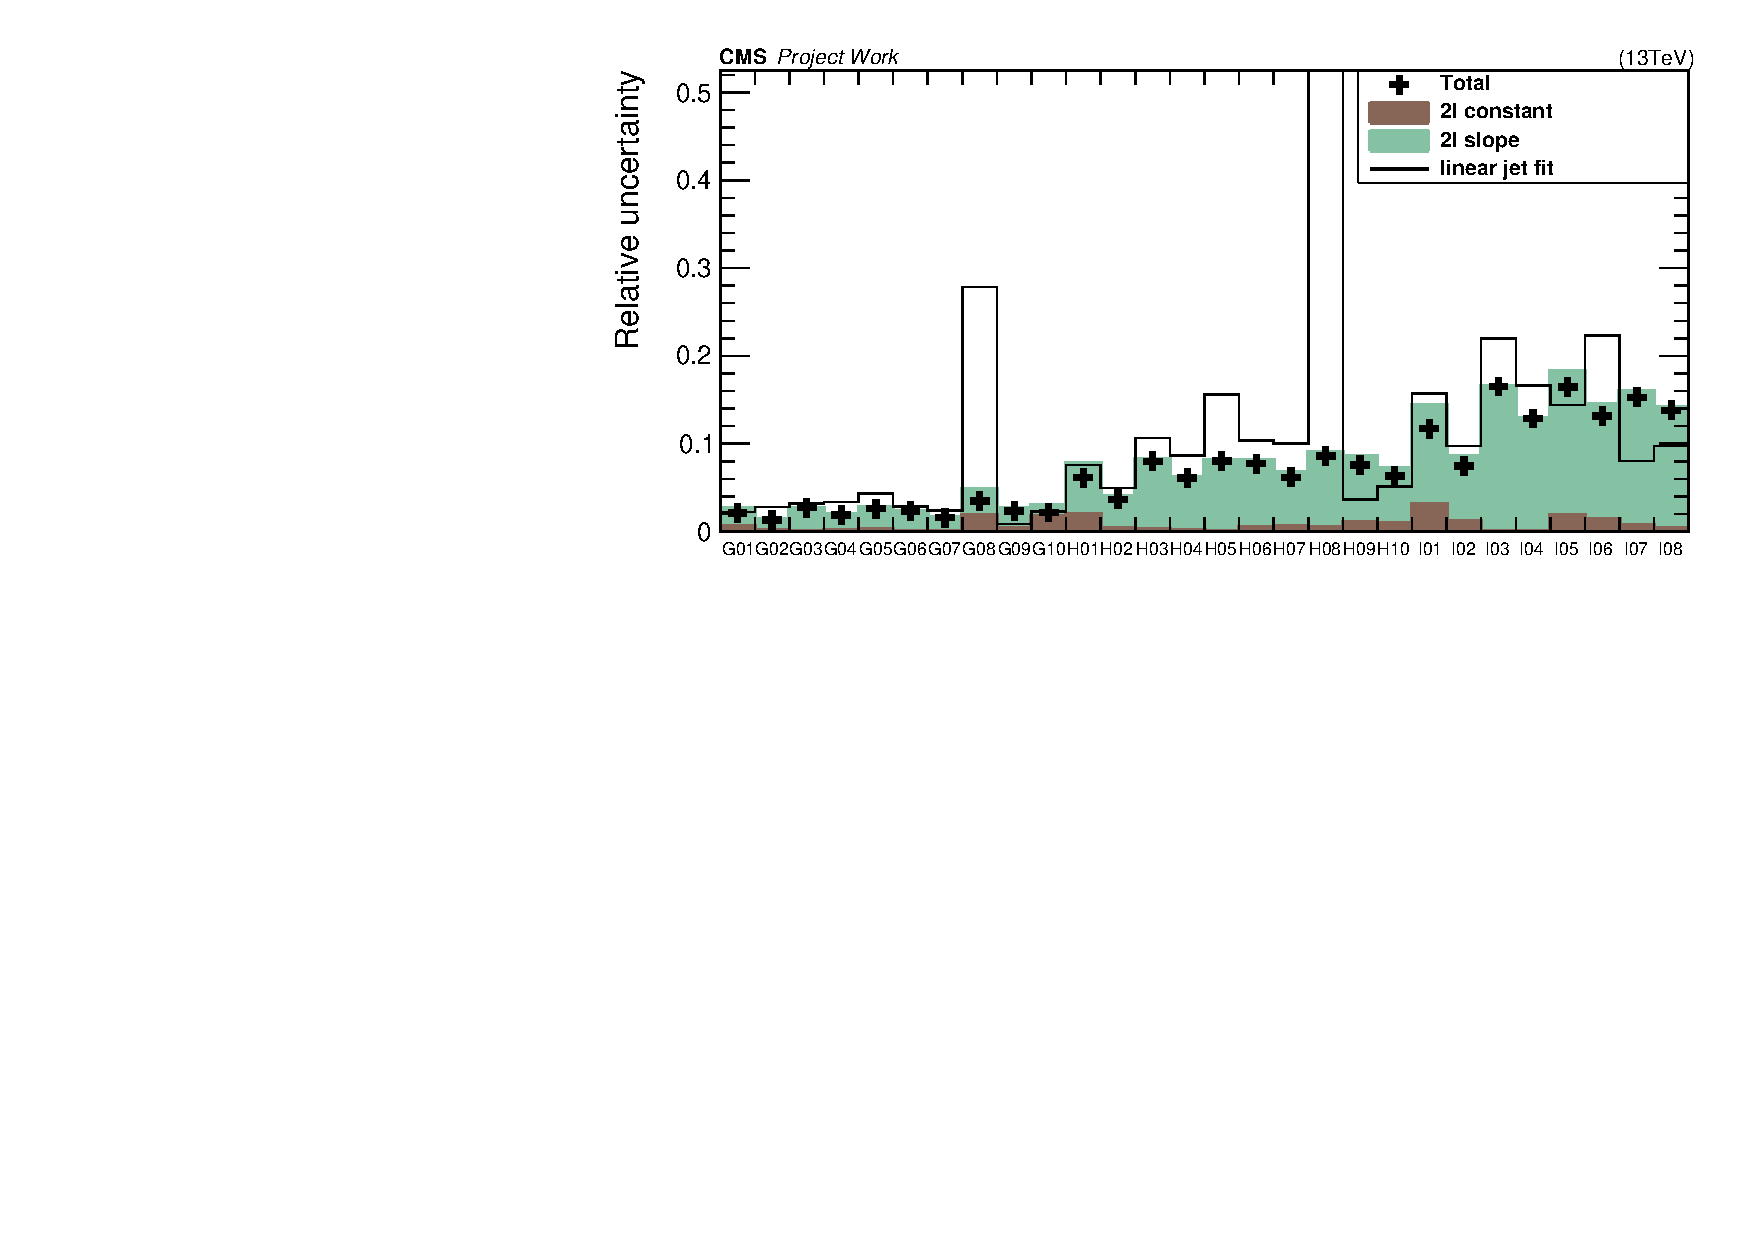
\includegraphics[width=0.95 \textwidth]{PhD_Thesis_v4/Plots/analysis/syst/dilepComp.pdf}
  \caption{ \label{fig:systDL} Relative uncertainty on $\kappa_{\ttbar}$ due to the different composition of dileptonic events in sideband and mainband regions. Color filled areas represent the dilepton uncertainties, while the black line shows the uncertainty which is calculated with a fit on the $\njet$ distribution.}
  \end{center}
\end{figure*}
\\
\textbf{Cross sections}\\
To account for possible biases in the estimation of the background composition in terms of $\wJets$ vs. $\ttJets$ events, uncertainties on their cross sections are taken in to account. Although the $W$ boson cross section and $\ttbar$ cross section uncertainties are at the order of ten percent level in the inclusive regions, they can be larger in the restricted phase space of the side bands. The $\wJets$ and $\ttJets$ cross sections are conservatively varied by $\pm$30\%, which leads to an average change of 0.3-10\% (0.7-13\%) in the $\kappa_w$ ($\kappa_{\ttbar}$) values. \\
For the smaller EWK background processes, which are taken from simulation, a conservative~50\% variation is applied. Because the fraction of these events are small, the effect of this variation on the $\kappa$ values is between~0.1-3.8\%.
\\
\textbf{W polarization}\\
The main search variable $\DF$ reflects the angular information between the W boson and its decay products. Therefore, the W boson polarization affects the $\DF$ distribution. The effect of the polarization on background estimation of $\wJets$ and $\ttJets$ is calculated by reweighting events according to the angle between the lepton and the leptonically decaying W boson in its rest frame within the uncertainties of the measured W boson helicity fractions~\cite{Wpol1,Wpol2}. The resulting  uncertainties are found to be below~3\%.
%is calculated by reweighing these events by:
%\begin{equation}
%\label{eqn:W_pol}
%\rm w = (1 \pm a\cdot(1-cos(\theta^*)))\cdot C
%\end{equation}
%where a is 5\% for  $\ttJets$ and 10\% for $\wJets$ events, C is a factor to keep the normalization after baseline constant and $\theta*$ is the angle between the charged lepton and the W boson in the W rest frame. This procedure results in an uncertainty below 3\% in all the signal regions. \\
\\
\textbf{ISR jet multiplicity}\\
In Sec.~\ref{sec:SF}, the reweighting of events according to number of ISR jets is already explained. $\kappa$ values are recalculated by varying the ISR weights with the systematic uncertainties listed in Tab.~\ref{tab:nISRweights}. The amount of variation is then estimated using the Eq.~\ref{eqn:syst_unc_kappa} and found to be ranging between~0.2-11\%.\\
\textbf{QCD multijet events prediction}\\
QCD multijet prediction is entering in this search via the b-tag multiplicity fit (see Sec.\ref{sec:bkgcomp}) to measure the background compositions in control regions. Therefore the uncertainty in the QCD multijet prediction has to be propagated. A profound explanation of the QCD prediction and its uncertainty can be found in \cite{David}. The effect of this uncertainty is propagated to the $\Rcs$ prediction. The resultant uncertainty is found to be approximately~3\% on $\kappa_w$ and $\kappa_{\ttbar}$.\\
\textbf{$\Rcs$ in the muon vs. the inclusive lepton selection}\\
As discussed in Sec.~\ref{sec:RcsW}, $\Rcs$ of $\wJets$ events is calculated only in the muon channel. To account for the inconsistency between the $\Rcs$ with only muon channel and the true $\Rcs$, the discrepancy between these values are taken from simulation. The discrepancy is assigned as systematic uncertainty. In order to avoid large uncertainties driven by the limited statistics, the estimated systematic uncertainty is constrained to be smaller than the statistical error on $\Rcs^{MC}$. \\
\section{Systematic uncertainties on signal modelling}
The uncertainties considered in this section are applied only to the simulated signal events. The amount of discrepancy is calculated as:
\begin{equation}
\label{eqn:syst_unc_signal}
\delta = \frac{N'_{\rm events}}{N_{\rm events}}-1\, ,
\end{equation}
where $N'_{\rm events}$ represents the recalculated number of simulated signal events with varied weights and $N_{\rm events}$ is the true number of events. The systematic uncertainties on the signals are calculated separately for each of the~657 gluino/neutrino mass points.\\
\textbf{Initial state radiation}\\
In Run 1, it was observed that the hadronic recoil from initial state radiation~(ISR) for boosted heavy particle pairs such as the $\ttbar$ system is not well described by the $\MADGRAPH$ event generator~\cite{ISR}. Because gluino pair production is also dominated by gluon fusion,
As a very similar system, it is expected that to be subject to a similar mismodeling.
An uncertainty based on the $\pt$ of the gluino-gluino system is applied:
\begin{itemize}
\item $\pt$ (gluino-gluino) less than 400~GeV: no uncertainty
\item $\pt$ (gluino-gluino) between~400 GeV and 600~GeV:~15\% uncertainty
\item $\pt$ (gluino-gluino) above 600~GeV:~30\% uncertainty.
\end{itemize}
The uncertainty on the number of expected signal events is calculated according to Eq.~\ref{eqn:syst_unc_signal}.\\
\textbf{Factorization/renormalization scale}\\
To account for the impact of renormalization and factorization scales on the signal acceptance, the scales are varied by a factor of~0.5 and~2, respectively. The cross section is kept constant and from the total of 8 possible variations, the anti-correlated ones are dropped. Then, an envelope of all variations is computed for each acceptance. The resultant uncertainty on the expected event yields is similar for all the mass points and it ranges between~1-3\%.\\
\textbf{Reconstruction of $\MET$} \\
FastSim signals are subject to $\MET$ mismodeling. In order to account for this effect, the yields are obtained based on $\MET$ and $\MET^{\rm gen}$, where the latter is obtained at generator level. Then, all kinematical observables are recalculated in the two cases, as well as the acceptances. The mean of the acceptances is taken as the central value and half of the difference is taken as systematic uncertainty. \\
\textbf{Trigger}\\
As shown in Sec.~\ref{sec:triggers}, the uncertainty on the trigger selection efficiency is measured to be approximately~2\%, and also considered as the uncertainty on signal simulation. \\
\textbf{Luminosity}\\
As shown in Sec.~\ref{sec:luminosity},  the pixel cluster counting method \cite{LUMTECH} is used to calculate luminosity. The uncertainty on this measurement is~2.5\%~\cite{lumi1}.\\
\section{Common systematic uncertainties for signal and background modelling}
Systematic uncertainties affecting both background and the signal processes are related to the mismeasurement or misidentification of particular objects in the events. These uncertainties have impact on the kinematic variables: $\DF$, $\LT$, $\HT$, $\njet$, $\nbjet$. Therefore, for the signal events they are affecting the acceptance and the selection efficiency and for the background events they may affect the $\Rcs$ values.\\
\textbf{Jet Energy Scale}\\
%Calculating uncertainty on the jet energy scales is another dedicated study performed by JET-MET physics object group at CMS. 
Variations of jet energy corrections within the uncertainties, which affect the jet energy spectrum as well as $\MET$, are applied to each jet in an event and therefore related kinematic variables,such as $\DF$, $\LT$, $HT$, $\njet$, $\nbjet$ are recalculated.\\
For the background estimate, $\kappa$ values are recalculated with up and down scaled jets. The uncertainty, which is obtained using Eq.~\ref{eqn:syst_unc_kappa}, is found to be varying between~0.7-26\%. For the signal, yields are recalculated and variation is measured using Eq.~\ref{eqn:syst_unc_signal}. In this case, depending on the mass point and signal region, uncertainty can take values up to~40\%.\\
\textbf{Tagging of b-jets}\\
B-tagging uncertainties, which are related to difference in b-tagging efficiency between simulated and observed events, have an influence through acceptance and b-tag multiplicity fit. Uncertainties are calculated to be less than~3\% for the background, and between~1-6\% for the signal.\\
\textbf{Lepton identification and reconstruction}\\
The differences in the identification and reconstruction efficiencies between the simulated and observed data events are evaluated using tag-and-probe methods~\cite{ELEID}. For the backgrounds, a flat~5\% uncertainty is assigned to account for this difference. For signal, additional uncertainties which originate from the difference between FastSim and full detector simulation are taken into account. The resulting uncertainty on the expected signal yields is found to be~2\%. \\
\textbf{Pileup}\\
To cover the difference between the simulated pileup and the one in data, the inelastic cross section is varied by~5\% up and down and the varied versions of~Fig.~\ref{fig:pileUpmine} is obtained. For the background, the varied weights are propagated to the $\kappa$ calculation. For the signal, due to the fact that the signal yields in MB SR do not significantly depend on pileup, FastSim samples are not reproduced for the high pileup environment. Nevertheless, a cross-check on the PU dependence of the two benchmark point is performed. The PU dependence is calculated as follows:
\begin{equation}
{\rm PU_{dependence}}= \frac{{\rm Efficiency_{high}} }{{\rm Efficiency_{low}} },
\end{equation}
where $\rm Efficiency_{high}$ and $\rm Efficiency_{low}$ is:
\begin{eqnarray}
\label{eff_PU}
{\rm Efficiency_{high}} = \frac{N(n_{\rm vertices}\geq20, {\rm MB})}{N(n_{\rm vertices}\geq20, {\rm baseline})},\nonumber\\
{\rm Efficiency_{low}} = \frac{N(n_{\rm vertices}<20, {\rm MB})}{N(n_{\rm vertices}<20, {\rm baseline})}.
\end{eqnarray}
\begin{figure*}[!hbt]
    \begin{center}
 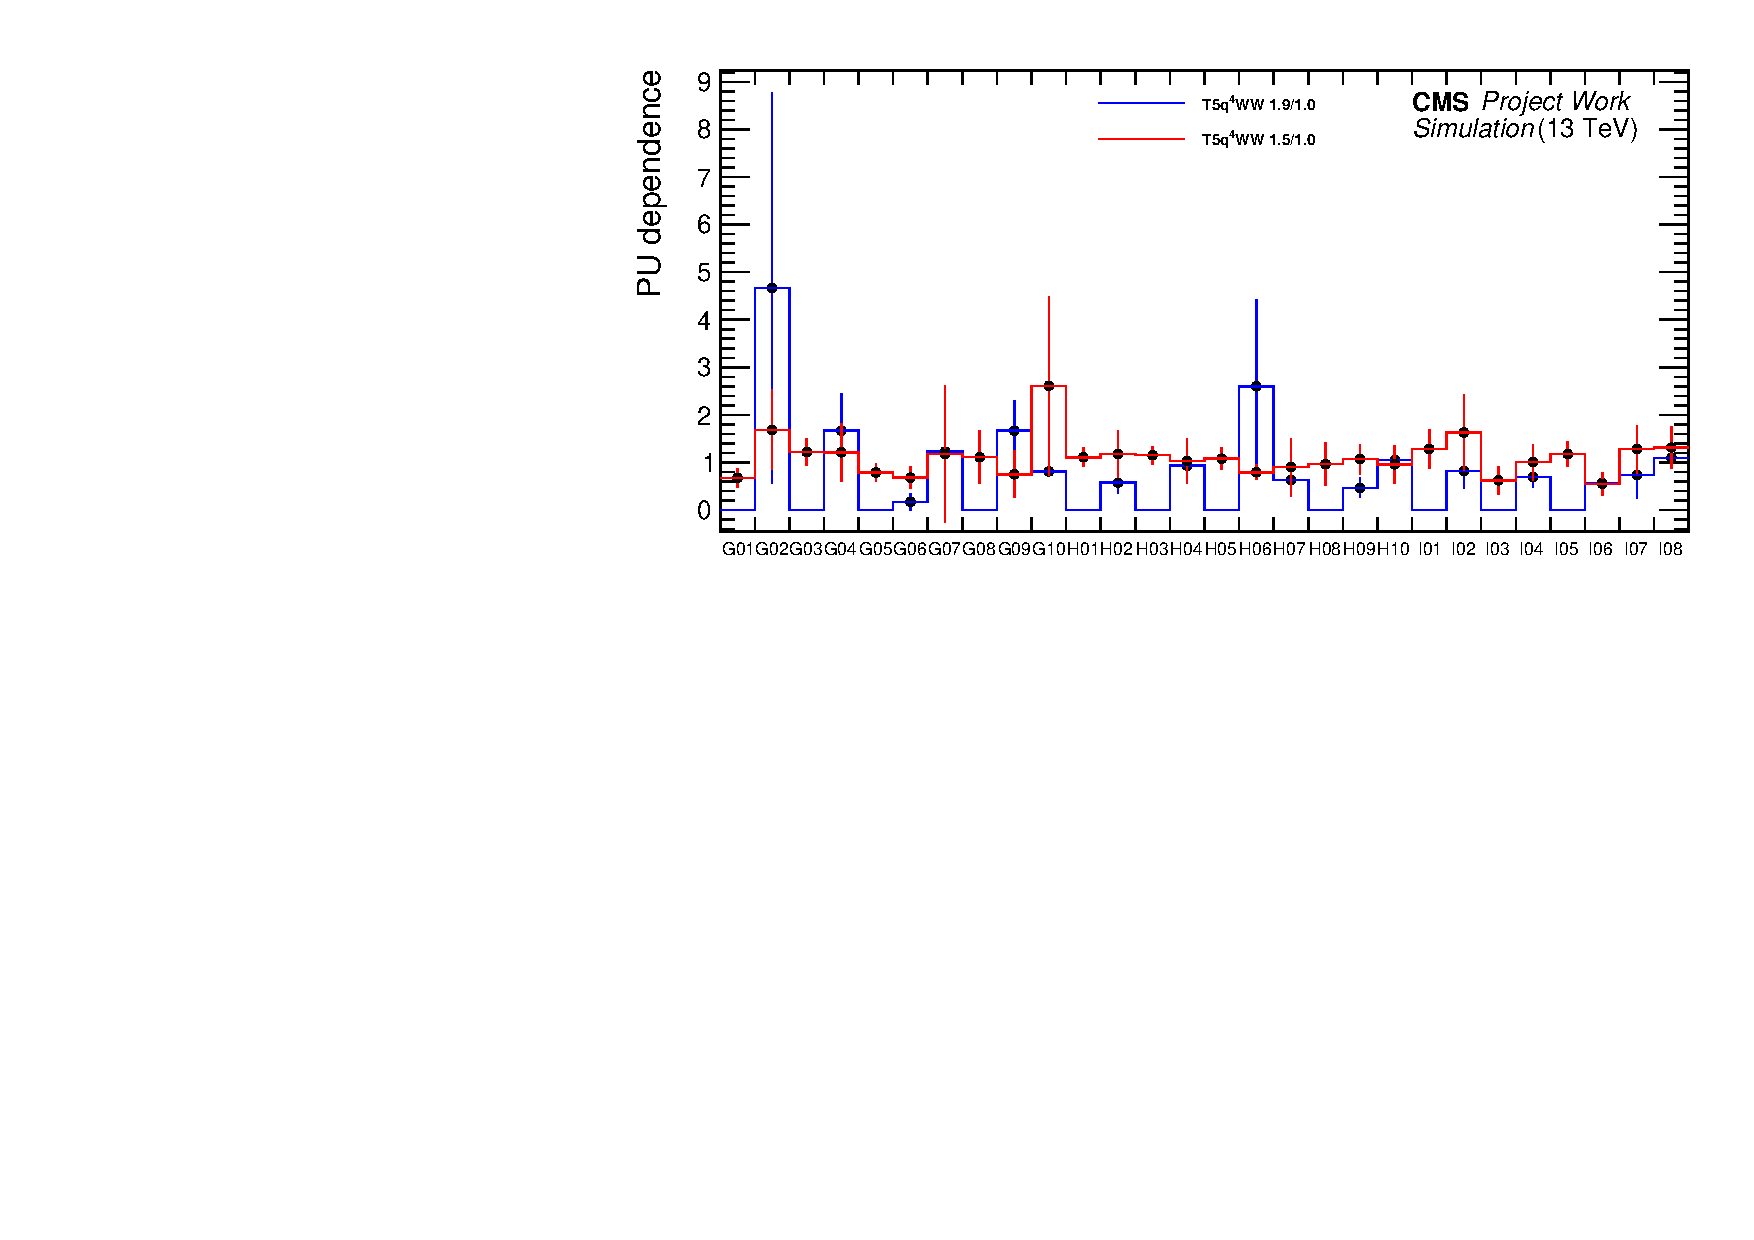
\includegraphics[width=0.8 \textwidth]{Plots/analysis/pileUp/PU_dependence}
  \caption{ \label{fig:pileUpdependence} Pileup dependence of the two signal benchmark points. The blue line is representing the high mass gap point the red one is for low mass gap region. The histogram points are following a flat line around 1.}
  \end{center}
\end{figure*}
The PU dependence as a function of search regions is shown in Fig.~\ref{fig:pileUpdependence}. 
The distribution is flat, therefore the uncertainty can be ignored.\\
However, still an uncertainty has to be assigned to cover the differences between the simulated signal pileup distribution and data, following steps have been employed. First, the signal sample is divided into a low and a high PU part according to mean value and then the mean values for each part is calculated as in Fig.~\ref{fig:pileUpsystmech}~(left).
Second, the simulated efficiency in MB SR is calculated for low and high pileup region as in Eq.~\ref{eff_PU}. Third, these four points, from first and second steps, together compose the two points in Fig.~\ref{fig:pileUpsystmech}~(middle). A linear fit is performed to extrapolate for all the pileup range. Finally, the data pileup distribution in Fig.~\ref{fig:pileUpsystmech} is normalized and folded with the fit and the sum is calculated. 
This procedure is repeated by varying the two values from second step within their statistical uncertainties independently.
The relative difference to the central value is taken as uncertainty.
Then, the uncertainty is separately obtained for low and high pileup region and combined in to one by taking the squared sum of the two. The entire procedure is repeated for each mass point in the gluino-neutralino mass plane and for each mainband region. The resulting uncertainty is found to be around~5-40\% depending on the statistics of the region for the corresponding mass point. In order not to double count the statistical errors, a~10\% flat uncertainty is applied to all bins for all mass points.\\
\begin{figure*}[!hbt]
    \begin{center}
  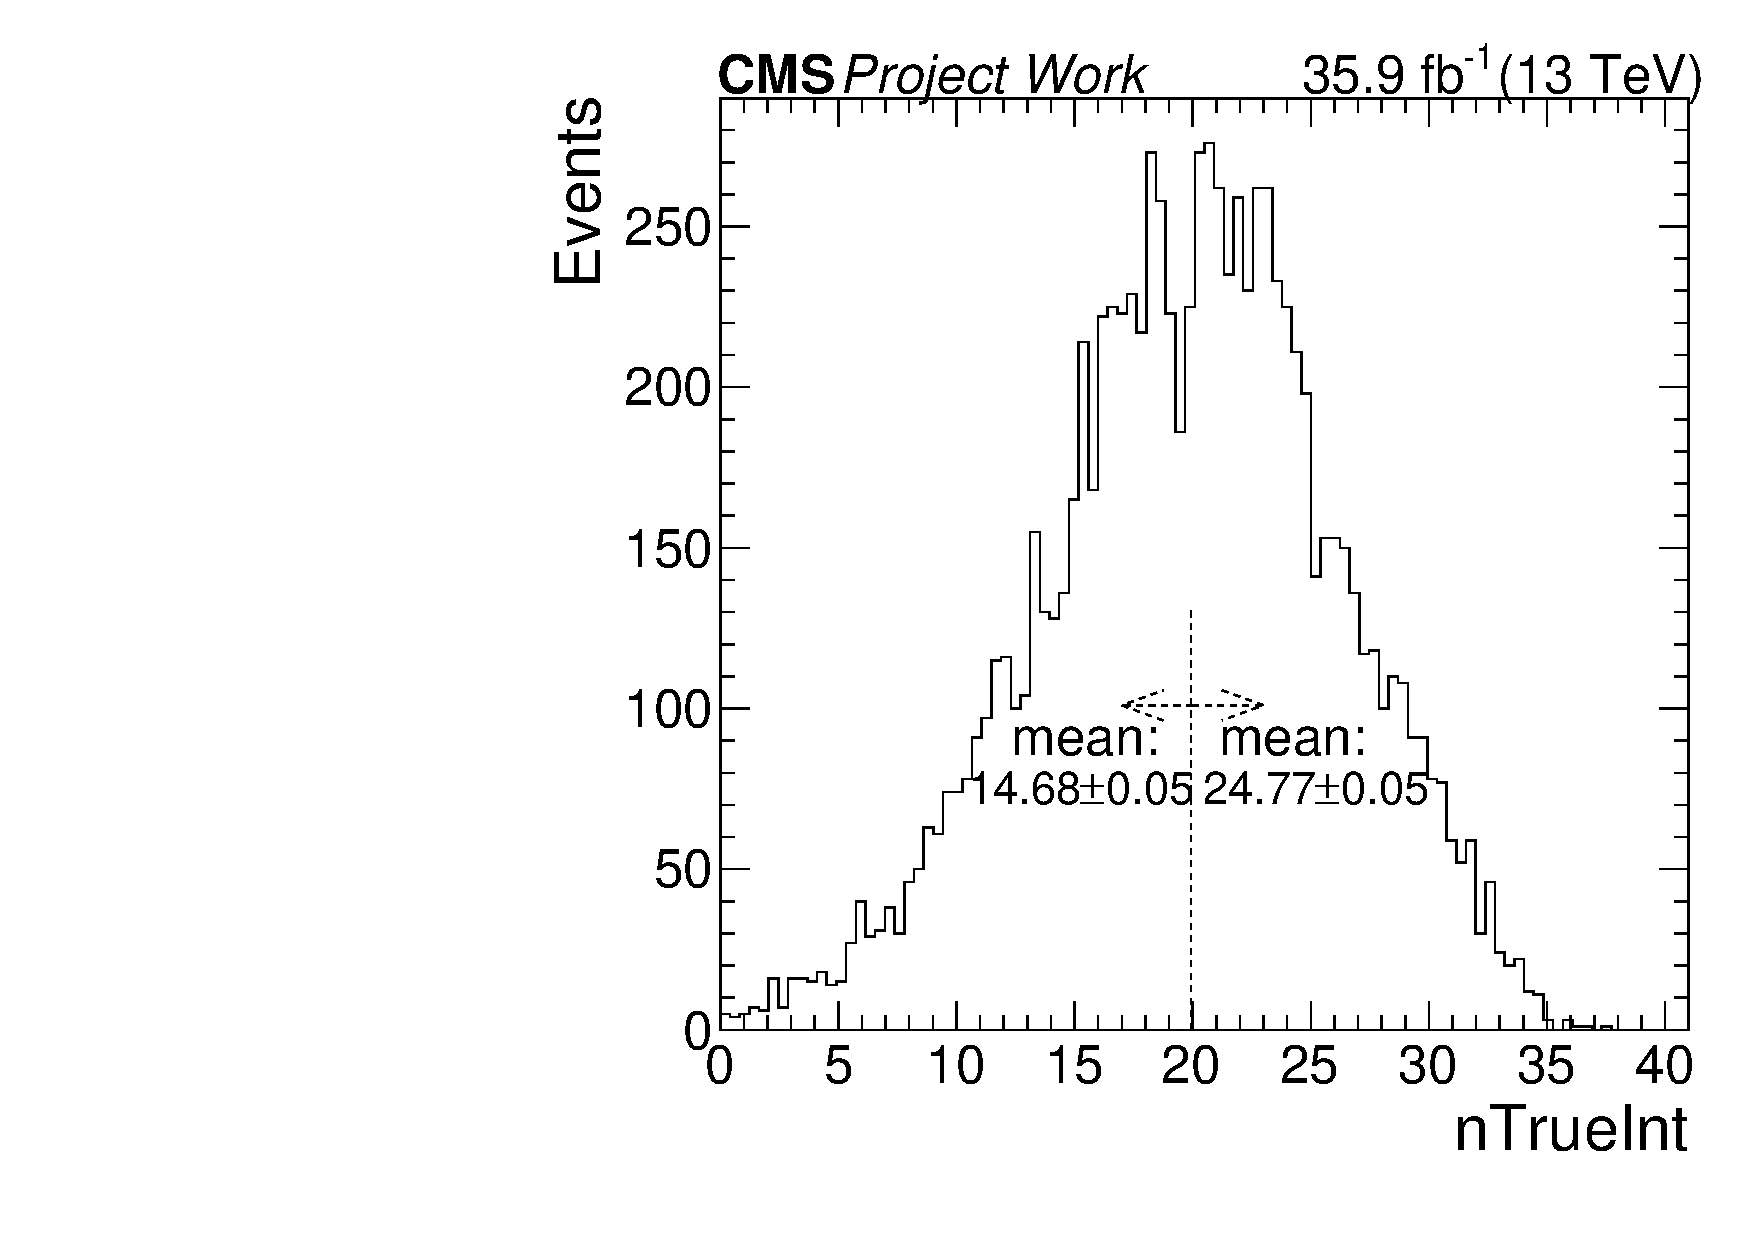
\includegraphics[width=0.28 \textwidth]{PhD_Thesis_v4/Plots/analysis/pileUp/1500_1000nTrueInt.pdf}
   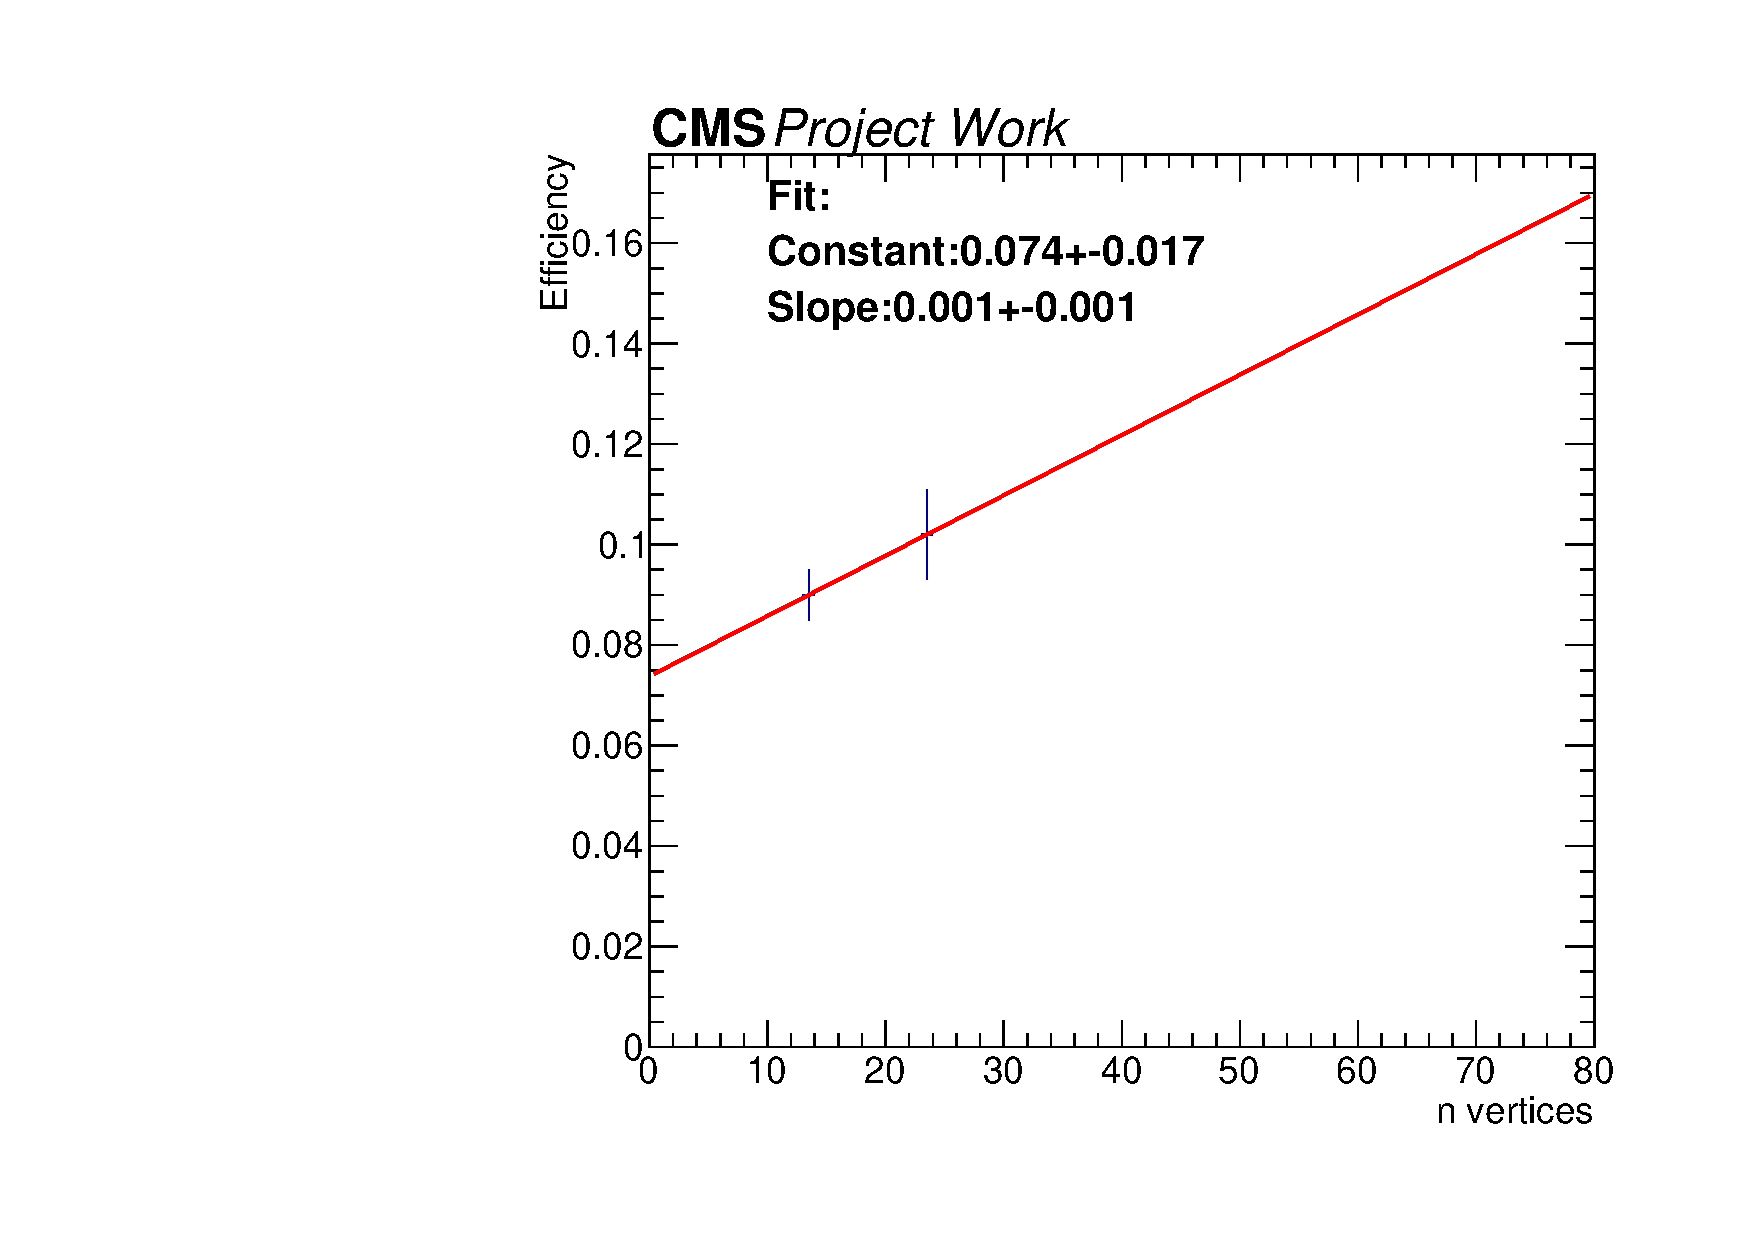
\includegraphics[width=0.3 \textwidth]{PhD_Thesis_v4/Plots/analysis/pileUp/PUFit.pdf}
    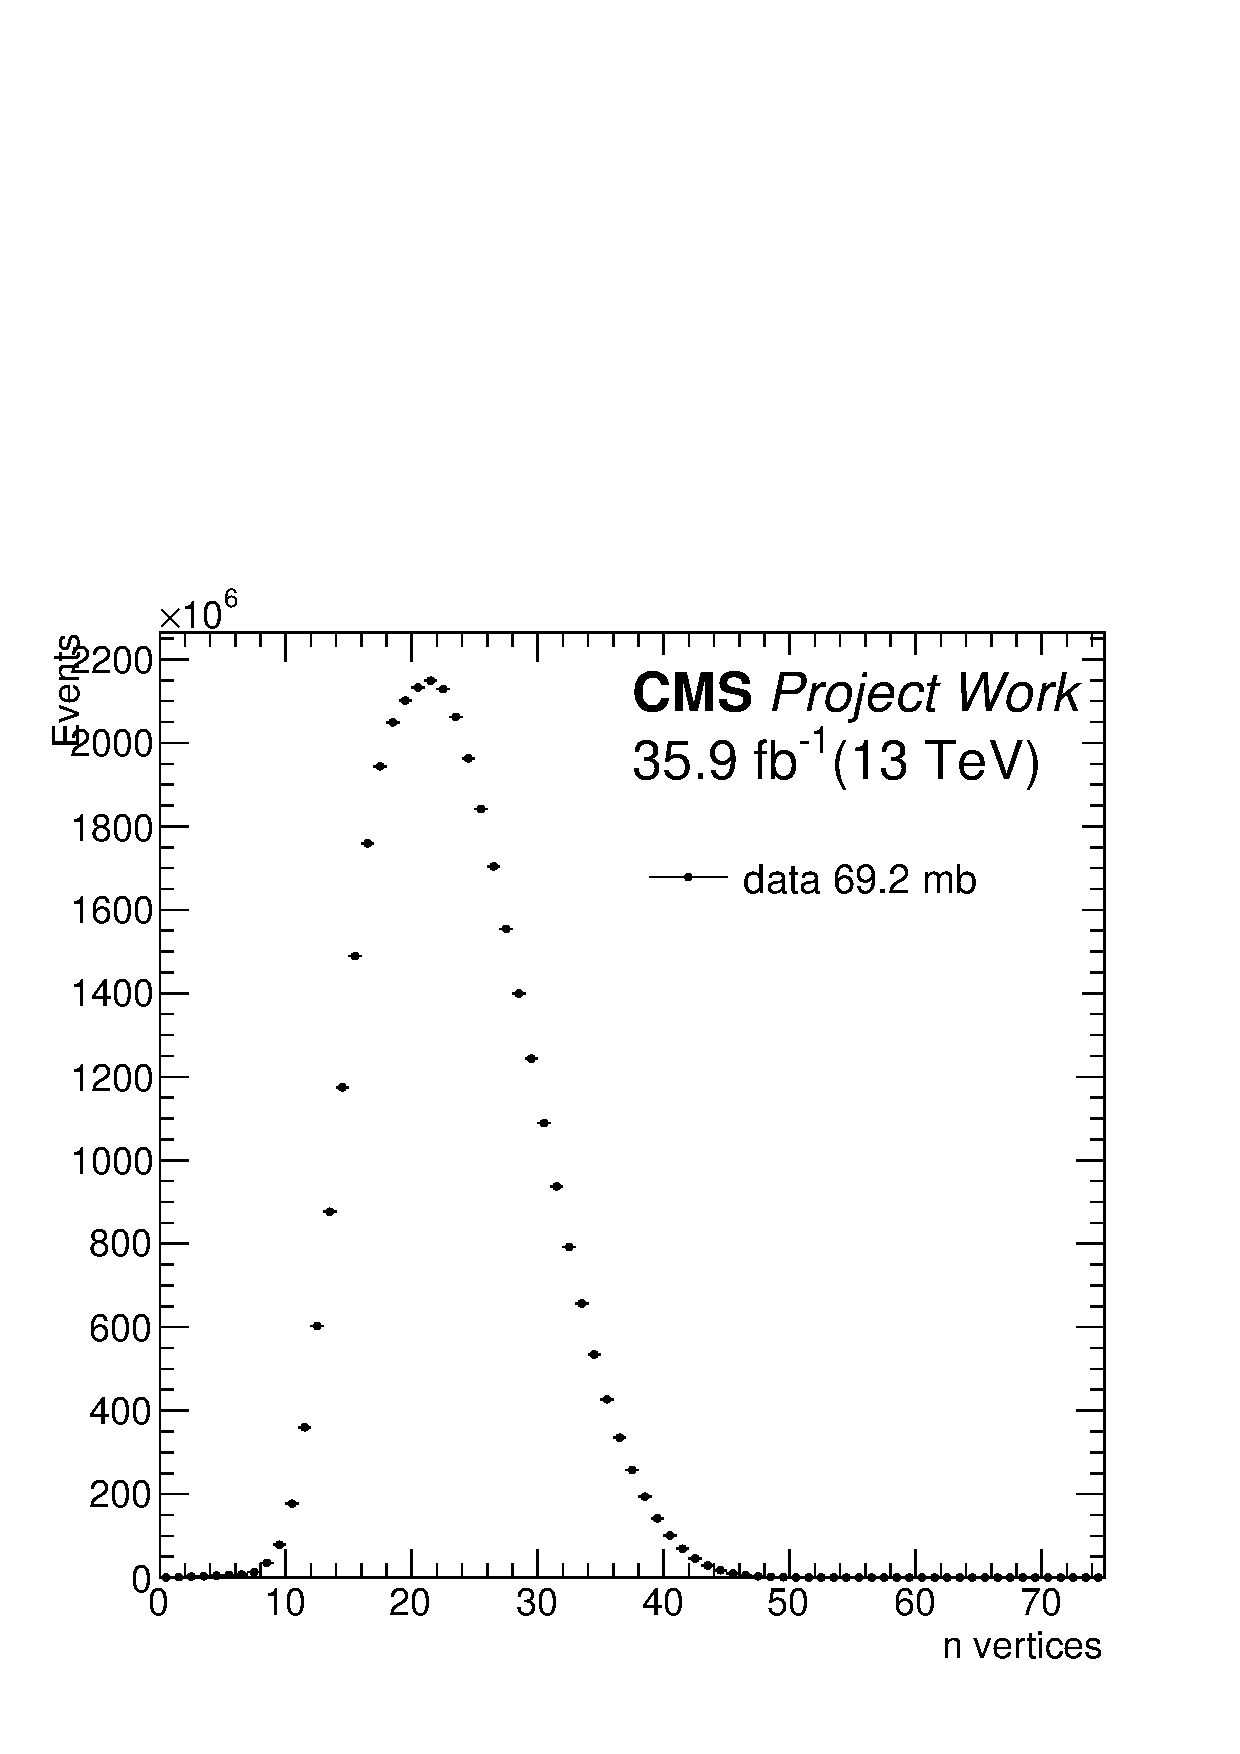
\includegraphics[width=0.28 \textwidth]{PhD_Thesis_v4/Plots/analysis/pileUp/histPUdata.pdf}
  \caption{ \label{fig:pileUpsystmech} Distribution of pileup for the low mass gap signal benchmark sample, divided in to two parts as low and high pileup region (left), example fit performed using the two points explained in the text (middle), data pileup  distribution which is folded with the fit.}
  \end{center}
\end{figure*}
\\
A summary of different systematic uncertainties on the background prediction for mainband signal regions are shown in Fig.~\ref{fig:systBKG}.
Moreover, a summary of the systematic uncertainties on the simulated signal events for the mass point $m_{\tilde{g}}=$~1900~GeV and $m_{\ninoone}=$~100~GeV is shown in Fig.~\ref{fig:systSig1}. The total systematic uncertainty is calculated as the squared sum of all the different sources are shown with the black crosses and they are just for illustration. The total systematic uncertainty and statistical uncertainties are shown in the lower band of the two figures.\\
\begin{figure*}[!hbt]
    \begin{center}
  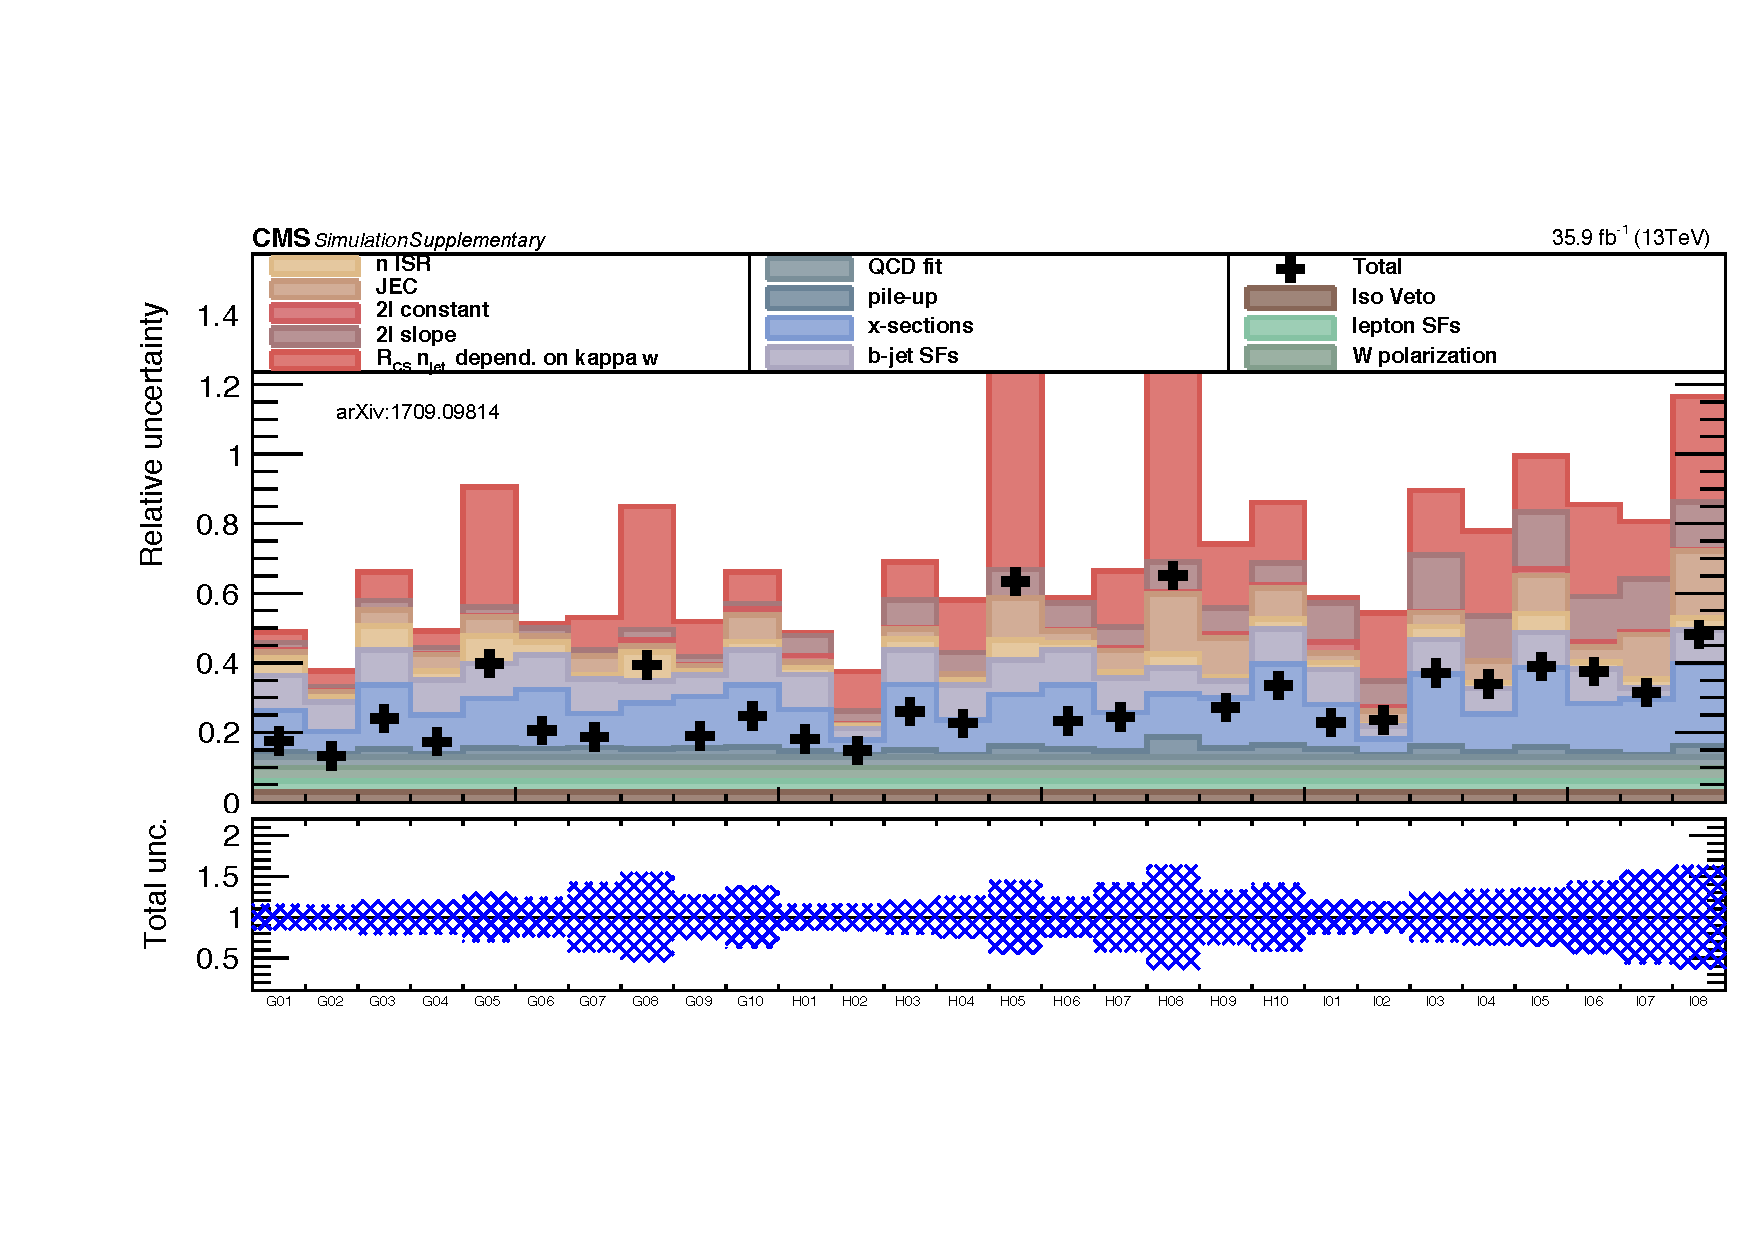
\includegraphics[width=0.9 \textwidth]{Plots/analysis/syst/plots_zerob_kappa_systematics_zerob}
  \caption[Summary of systematic uncertainty for background prediction]{ \label{fig:systBKG} Visualization of all systematic uncertainties~(upper panel) on the background prediction for mainband regions which are described in Tab.~\ref{tab:Sim_results}. The black crosses show an approximate total systematic uncertainty. They show the squared sum of all the different sources which are scaled according to their contribution. The total systematic uncertainty and statistical uncertainties are shown in the lower band.}
  \end{center}
\end{figure*}
\begin{figure*}[!hbt]
    \begin{center}
  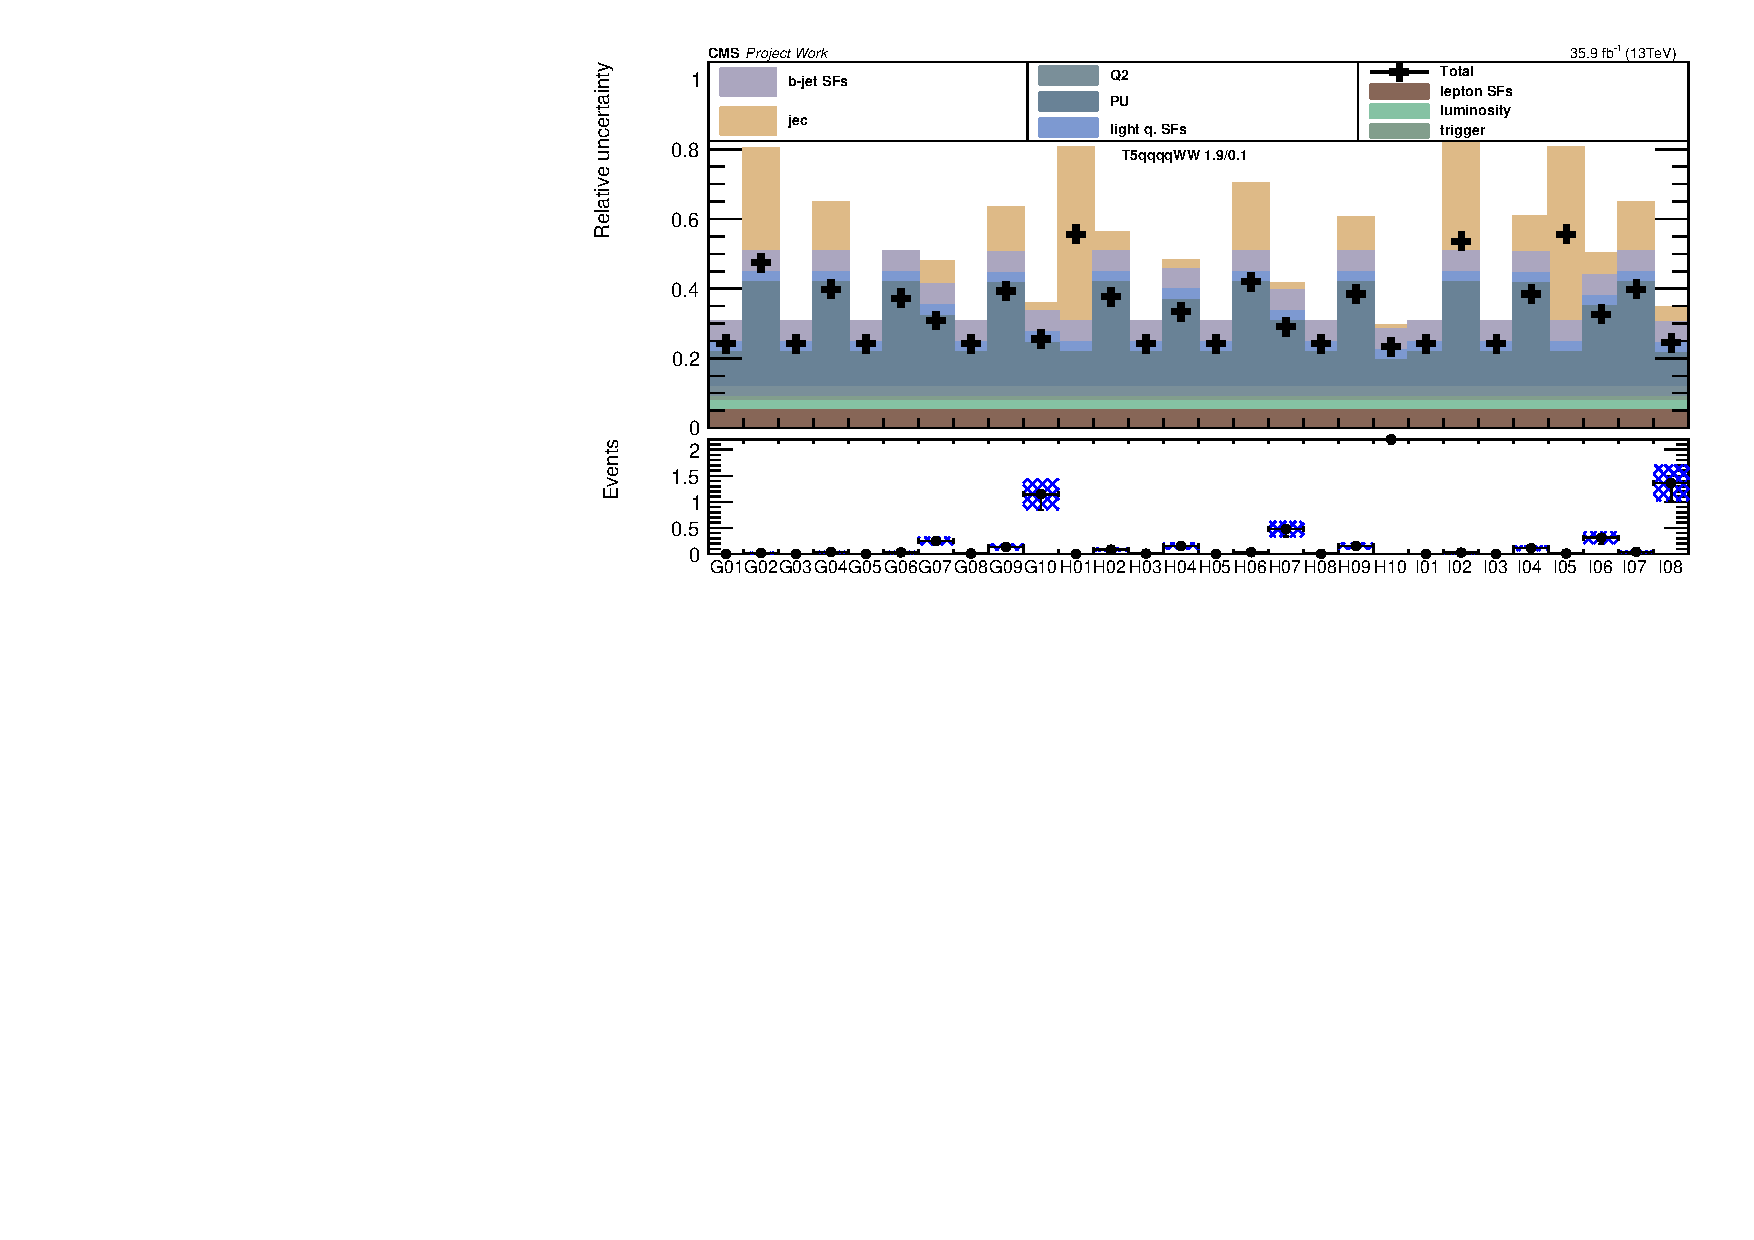
\includegraphics[width=0.9 \textwidth]{PhD_Thesis_v4/Plots/analysis/syst/sys_signal.pdf}
\caption[Summary of systematic uncertainty for signal simulation.]{ \label{fig:systSig1} Visualization of all systematic uncertainties~(upper panel) on the simulated signal yields in main band regions described in Tab. \ref{tab:Sim_results}. Uncertainties are shown only for one mass point which is  $m_{\tilde{g}}=$~1900 and $m_{\ninoone}=$~100. The lower panel shows the event counts with the total systematic and statistical uncertainty~(blue shaded area) on the yields.}
  \end{center}
\end{figure*}
